%%
%% 研究報告用スイッチ
%% [techrep]
%%
%% 欧文表記無しのスイッチ(etitle,jkeyword,eabstract,ekeywordは任意)
%% [noauthor]
%%

\documentclass[submit,techrep]{ipsj}
%\documentclass[submit,techrep,noauthor]{ipsj}



\usepackage[dvips]{graphicx}
\usepackage{latexsym}
\usepackage[dvipdfmx]{}

\def\Underline{\setbox0\hbox\bgroup\let\\\endUnderline}
\def\endUnderline{\vphantom{y}\egroup\smash{\underline{\box0}}\\}
\def\|{\verb|}

\setcounter{巻数}{58}%vol53=2012
\setcounter{号数}{10}
\setcounter{page}{1}


\begin{document}


\title{マルチテナントシステムの開発を支援するIaaS環境}

\etitle{IaaS environment to support multi-tenant system development}

\author{古橋 健斗}{Kento Furuhashi}{Shibaura Institute of Technology}[ma17099@shibaura-it.ac.jp]
\author{松本 拓也}{Takuya Matsumoto}{Shibaura Institute of Technology}
\author{福田 浩章}{Hiroaki Fukuda}{Shibaura Institute of Technology}[hiroaki@shibaura-it.ac.jp]

\begin{abstract}
クラウドサービスでは,アプリケーションを提供するサービス提供者が物理マ
シンやネットワークを保有するインフラ提供者から必要に応じてリソース
(e.g., 仮想マシン)を確保し,サービスを提供している.サービス提供者は,
最大負荷(必要になる仮想マシンの最大数)を見積もることでサービスの円滑な
運用を目指しているが,予め見積もることは難しい.一方,インフラ提供者は,
物理マシン,仮想マシンの負荷状況(e.g, CPUやメモリ使用量)をもとに仮想マ
シンを再配置し,データセンタ全体の運用効率向上を目指している
\cite{cloud1}\cite{cloud2}.この検証には実運用に適用することが望ましい
が,サービス提供者のSLAを保証する必要があり,実現は難しい.また,大規
模なデータセンタを準備することも難しいため,シミュレーションでの検証を
行わざるをえない\cite{testbed}.そこで本研究では,RaspberryPIを利用し,
サービス提供者,インフラ提供者それぞれの要求を容易にテストできる環境を
提供する.具体的には,複数のRaspberryPIを使用した仮想データセンタの構
築と負荷状況の監視,仮想マシンの操作を実現する.また,必要に応じて仮想
マシンを増減し,スケールアウトする機能を実現する.そして,仮想マシンの
移動,スケールアウトを本環境で実行し,その機能性能を示す.
\end{abstract}

%
%\begin{jkeyword}
%情報処理学会論文誌ジャーナル,\LaTeX,スタイルファイル,べからず集
%\end{jkeyword}
%
%\begin{eabstract}
%This document is a guide to prepare a draft for submitting to IPSJ
%Journal, and the final camera-ready manuscript of a paper to appear in
%IPSJ Journal, using {\LaTeX} and special style files.  Since this
%document itself is produced with the style files, it will help you to
%refer its source file which is distributed with the style files.
%\end{eabstract}
%
%\begin{ekeyword}
%IPSJ Journal, \LaTeX, style files, ``Dos and Dont's'' list
%\end{ekeyword}

\maketitle

%1
\section{はじめに}
仮想化技術の進化を背景に,物理マシンを保有してサービスを展開する形態
(シングルテナント)から,必要に応じてリソース(e.g., CPUやメモリ)を確保
しサービスを展開する形態(マルチテナント)に移行している.そして,これら
はAmazon Web Service~(AWS)やMicrosoft Azureのようなクラウドサービスを
利用して提供されている.マルチテナント環境では,図\ref{fig:user}に示す
ようにアプリケーションを提供するサービス提供者が物理マシンやネットワー
クを保有するインフラ提供者から必要に応じてリソース(e.g., 仮想マシン)を
確保し,サービスを提供している.サービス提供者は,最大負荷(必要になる
仮想マシンの最大数)を見積もることでサービスの円滑な運用を試みるが,予
め正確に見積もることは難しい.
そのため,実際には経験に基づき最大数を設定し,運用している.
一方,インフラ提供者は,物理マシン,仮想
マシンの負荷状況(e.g, CPUやメモリ使用量)をもとに仮想マシンを再配置し,
データセンタ全体の運用効率向上を目指している\cite{cloud1}\cite{cloud2}.
この検証には実運用に適用することが望ましいが,サービス提供者のSLAを保
証する必要があり,実現は難しい.また,大規模なデータセンタを準備するこ
とも難しいため,シミュレーションでの検証を行わざるをえない\cite{testbed}.

一方,近年小型計算機の開発を背景に,それらを複数台利用してクラスタとして利用する事例や,
SDNの検証に用いる例が見受けられる.小型計算機は一般の計算機やサーバと比較して安価で,
複数台用意することも十分に可能である.また,仮想化機能を備えたCPUを搭載する小型計算機
も存在する.

そこで本研究では,小型計算機の一つであるRaspberryPI(RasPI)を利用してデータセンタを模擬し,
インフラ提供者が効率の良いデータセンターの運用方式(e.g., アルゴリズム)を開発するテスト環境を提供する.
また,予め最大数を見積もることなく,物理マシン,仮想マシンの状況に応じて動的に仮想マシンを複製し,
動的に負荷を分散する機構(オンデマンドスケールアウト)を実現する.
そして,負荷分散や運用効率を判定する指標となるCPUやネットワークの負荷の取得する機能,および仮想マシンの複製や
移動を実行する機能をAPIとして提供する.
最後に,これらのAPIを使用して仮想マシンの移動,スケールアウトを実行し,テスト環境の基本性能を示す.

以降,2節では本研究で想定するクラウド環境について概説し,テスト環境の要件を整理する.
3節では本研究のアプローチについて概説し,4節で
実装について述べる.次に5節ではテスト環境での実験と結果をまとめる.
そして,6節で関連研究について述べ,最後7節でまとめと今後の課題を述べる.

\begin{figure}[tb]
	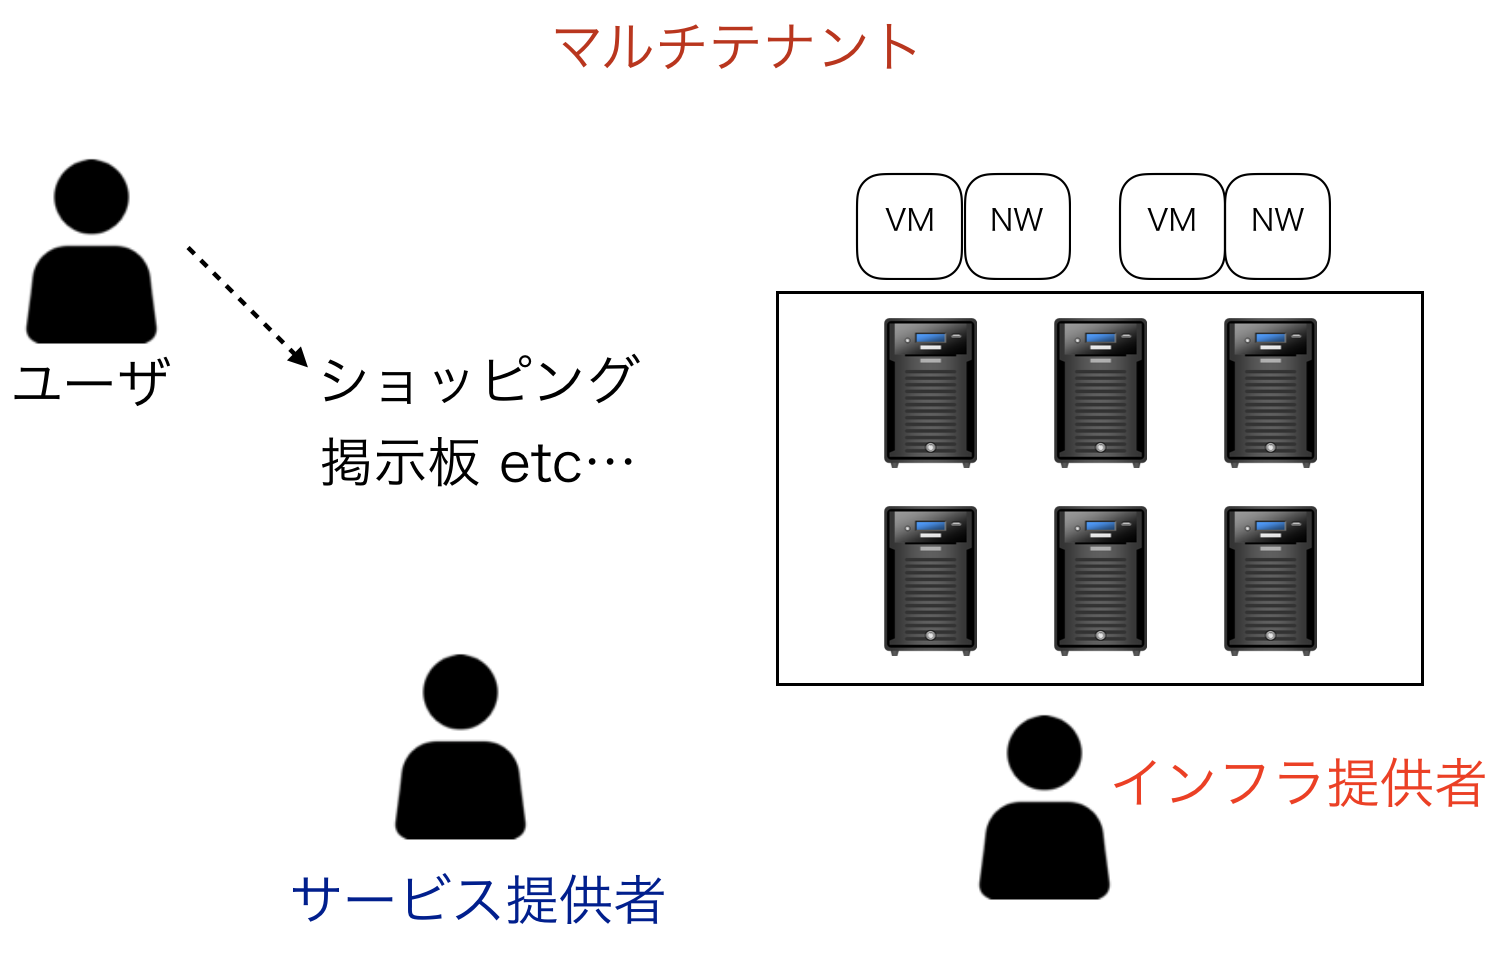
\includegraphics[width=8.5cm,bb=0 0 941 514]{fig/user.png}
	\caption{マルチテナント環境}
	\label{fig:user}
\end{figure}

\section{クラウド環境とテスト環境の要件}
本節では,本研究で想定するクラウド環境を概説し,それらの実現に必要なテスト環境の要件を述べる.
\begin{figure}[tb]
	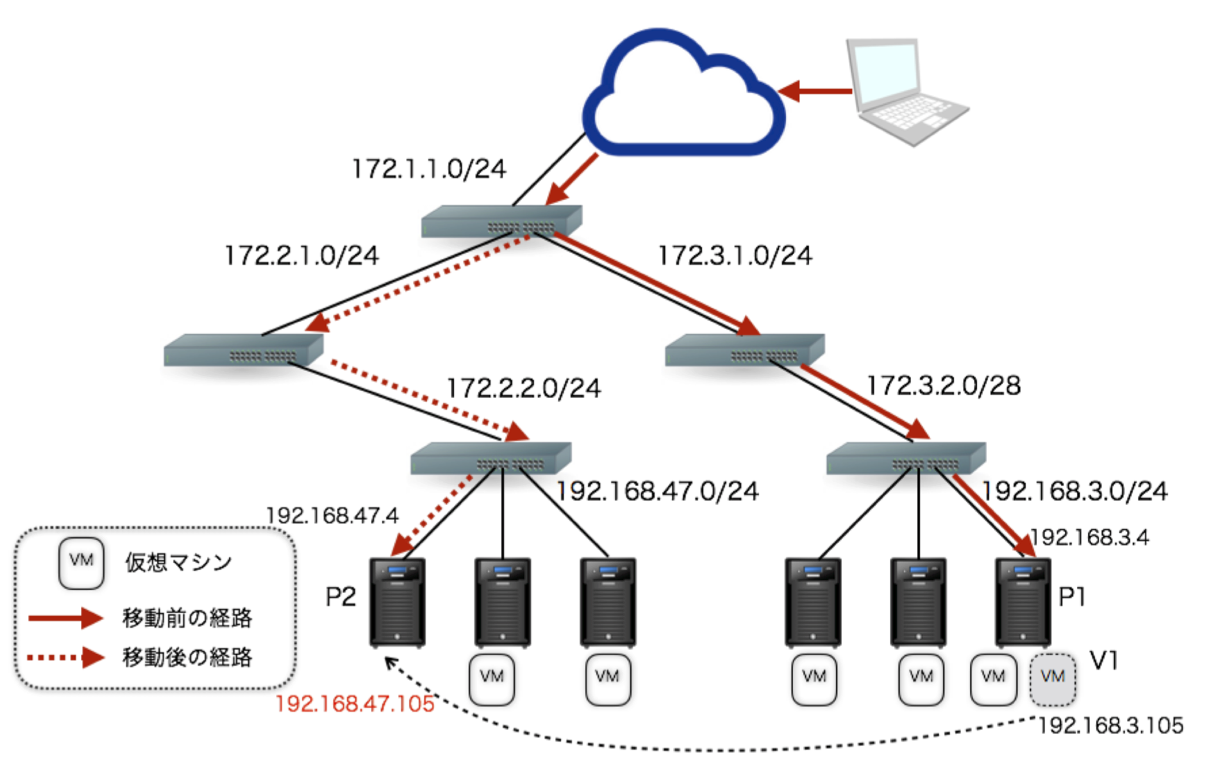
\includegraphics[width=8.5cm,bb=0 0 579 366]{fig/cloud.png}
	\caption{想定するクラウド環境}
	\label{fig:cloud}
\end{figure}

\subsection{クラウド環境}\label{subsec:cloud}
本研究で想定するクラウド環境を図\ref{fig:cloud}に示す.クラウド環境で
は,一般に複数のネットワークスイッチとそれらに接続した物理マシンで構成
される.そして,サービス提供者からリソース取得の要求があると,インフラ
提供者は物理マシンで仮想マシンを起動してそれらを提供している.クライア
ントのリクエストはスイッチで適切に転送され,対象となる仮想マシンが適切
に処理してサービスを運用している.ここで,物理マシンが高負荷になり,仮
想マシンを移動する状況を想定する~(図\ref{fig:cloud}).図
\ref{fig:cloud}では,物理マシンP1で仮想マシンV1が動作している状況にお
いて,V1を物理マシンP2に移動することを想定している.P1とV1にはそれぞれ
IPアドレス(192.168.3.4, 192.168.3.105)が設定されており,ユーザの立場か
らは区別できない.一方,P2にも192.168.47.4のIPアドレスが設定されている.
仮想マシンの移動では,一般にIPアドレスは変化しないため,V1のIPアドレス
はP2に移動した後も変わらず192.168.3.105となる.V1の移動はP2が直接接続
しているネットワークスイッチ,および上流に位置するスイッチに影響しない
ため,従来V1に届けられていたパケットは依然として192.168.3.0/24を管理す
るスイッチに届けられることになり,移動後のV1に届けられることはない.移
動後のV1に正しくパケットを届けるためには,V1のIPアドレスと移動後のネッ
トワークに合致したものに変更(e.g., 192.168.47.105)する必要がある.加え
て,ユーザからはこの変更は透過であるため,V1へのリクエストは依然として
192.168.3.105宛に送信される.しががって,ネットワークスイッチに変更を
加え,宛先192.168.3.105へのパケットは変更後のアドレスに書き換えて
(192.168.47.105)送信する必要がある.

このように,クラウド環境で円滑にサービスを運用するためには,仮想マシンの移動や
複製に伴い,関連するネットワークスイッチも連動して変更する必要がある.

\subsection{テスト環境の要件}\label{subsec:requirement}
\ref{subsec:cloud}節で述べたように,本研究で想定するクラウド環境の実現には,
仮想マシンの移動だけでなく,IPアドレスの変更など,移動に伴う変更や,移動の契機となる
状況の把握,多数のマシンを制御できる必要がある.
本研究では,クラウド環境を実現するため,以下の項目をクラウド環境の必要要件
と考える.

\begin{description}
\item [負荷状況の把握]仮想マシンの移動や複製は,一般に高負荷状態にある
  物理マシンの負荷を分散し,仮想マシンで提供するサービスの性能維持や,
  低負荷状態の物理マシンに散財する仮想マシンを集約し,リソースの効率的
  な使用ののために行われる.本テスト環境でもこれらの負荷状態を測定する
  ため,負荷状態の判定に一般的に用いられるCPUとメモリ使用率を使用する.
  また,物理マシンの負荷分散を目的として仮想マシンを移動させる場合,移
  動先物理マシンを決定する必要があるが,ネットワークを利用したサービス
  に主に用いられるクラウド環境ではネットワーク使用量も移動先を決定する
  指標となり得る.そこで本研究では,物理マシン単体のネットワーク使用量
  だけでなく,スイッチ単位でのネットワーク使用量を測定し,移動先決定の
  指標に用いる.

\item [IPアドレスとルーティング管理]仮想マシンが移動する時,移動先物理マシンが同一
  ネットワークに所属している場合にはIPアドレスの変更は必要ない.しかし,
  \ref{subsec:cloud}節でも述べたように,異なるネットワークに所属する物
  理マシンに移動する場合には移動後にIPアドレスの変更が必要になる.同一
  ネットワーク内だけの移動/複製は,クラウド環境の効率的な運用の妨げに
  なるため,本研究ではネットワーク間を跨いだ仮想マシンの移動/複製も想定
  する.その場合,複数の物理/仮想マシンに同一のIPアドレスを指定するこ
  とはできないため,仮想マシン移動時にはIPアドレスを開放し,移動後には
  未使用のIPアドレスを設定できる必要がある.
  さらに,ネットワーク間を跨いだ仮想マシンの移動/複製には,\ref{subsec:cloud}節で述べたように,
  IPアドレスの変更に伴い,関連するネットワークスイッチを変更し,適切にクライアントからのリクエストを
  転送する必要がある.

\item [複数マシンの管理]本研究では,クラウド環境の効率的な運用のため,
  仮想マシンの移動/複製を効率的に行うアルゴリズム開発/検証にテスト環境
  を利用することを想定している.そのため,本テスト環境は多数の物理マシ
  ン,ネットワークスイッチで構成することになり,それぞれの状態管理
  (e.g, 負荷の測定)や制御(e.g, 設定変更や仮想マシンの移動/複製)を個別
  に行うことは現実的には難しい.そこで,テスト環境を構成する物理マシン
  やネットワークスイッチを一元管理し,設定変更や制御を用意に実現できる
  必要がある.
  
\end{description}

\section{テスト環境の実現}
本節では,RasPIで仮想環境を実現する方法について述べた後,
\ref{subsec:requirement}節で挙げた要件に対応する本研究での実現方法を述
べる.

\begin{table}[tb]
	\centering
	\caption{RaspberryPi2 ModelBの性能}
	\label{tab:rpi2}
	{
		\small
		\begin{tabular}{|c|c|} \hline
		CPU & ARM Cortex-A7 クアッドコア 900MHz\\ \hline
		メモリ & 1GB\\ \hline
		ネットワーク & 10/100Mbpsイーサネット\\ \hline
		電源 & 900mA(4.5 \textasciitilde 5.5W)\\ \hline
		\end{tabular}
	}
\end{table}

\subsection{RaspberryPIでの仮想化環境}
本研究のテスト環境では\ref{tab:rpi2}に示すRaspberryPI2 ModelBを利用し,
Linux系専用OSであるRaspbian Jessie Liteを実行する.CPUであるARM
Cortex-A7は仮想化拡張機能を備えているため,Linuxカーネルが備えるハイパー
バイザ,KVMを実行することができる.一般のPCでは,KVMはパッケージ管理ソ
フトウェア(e.g., apt-get)などを利用してインストールできるが,RasPIでは
パッケージでは提供されていない.そのため,カーネルの組み込み機能として
実行する.また,KVMでの仮想マシンの管理にはvirt\cite{virt}を利用することが
一般的であるが,RasPIではvirtを利用することができない.そのため,本研
究ではKVMと連携して動作するqemuが提供するコマンドを利用する.

一方,\ref{subsec:requirement}節でも述べたように,本テスト環境の実現に
は仮想マシンの移動/複製に同期したネットワークの変更が必要になる.近年,
仮想化技術の進歩に伴い,ネットワークを柔軟に制御するためにSoftware
Defined Network~(SDN)\cite{sdn}が注目を集めており,利用されている.そ
こで本研究でもSDNを利用してネットワークを制御する.本研究ではSDNの一種
であり,広く利用されているOpenFlow\cite{opf}を利用するため,OpenFlow対
応のソフトウェアスイッチであるOpen vSwitch(OvS)をRasPIにインストールし
て利用する.そのため,本テスト環境はすべてRasPIだけで構成できる.

\begin{figure}[tb]
	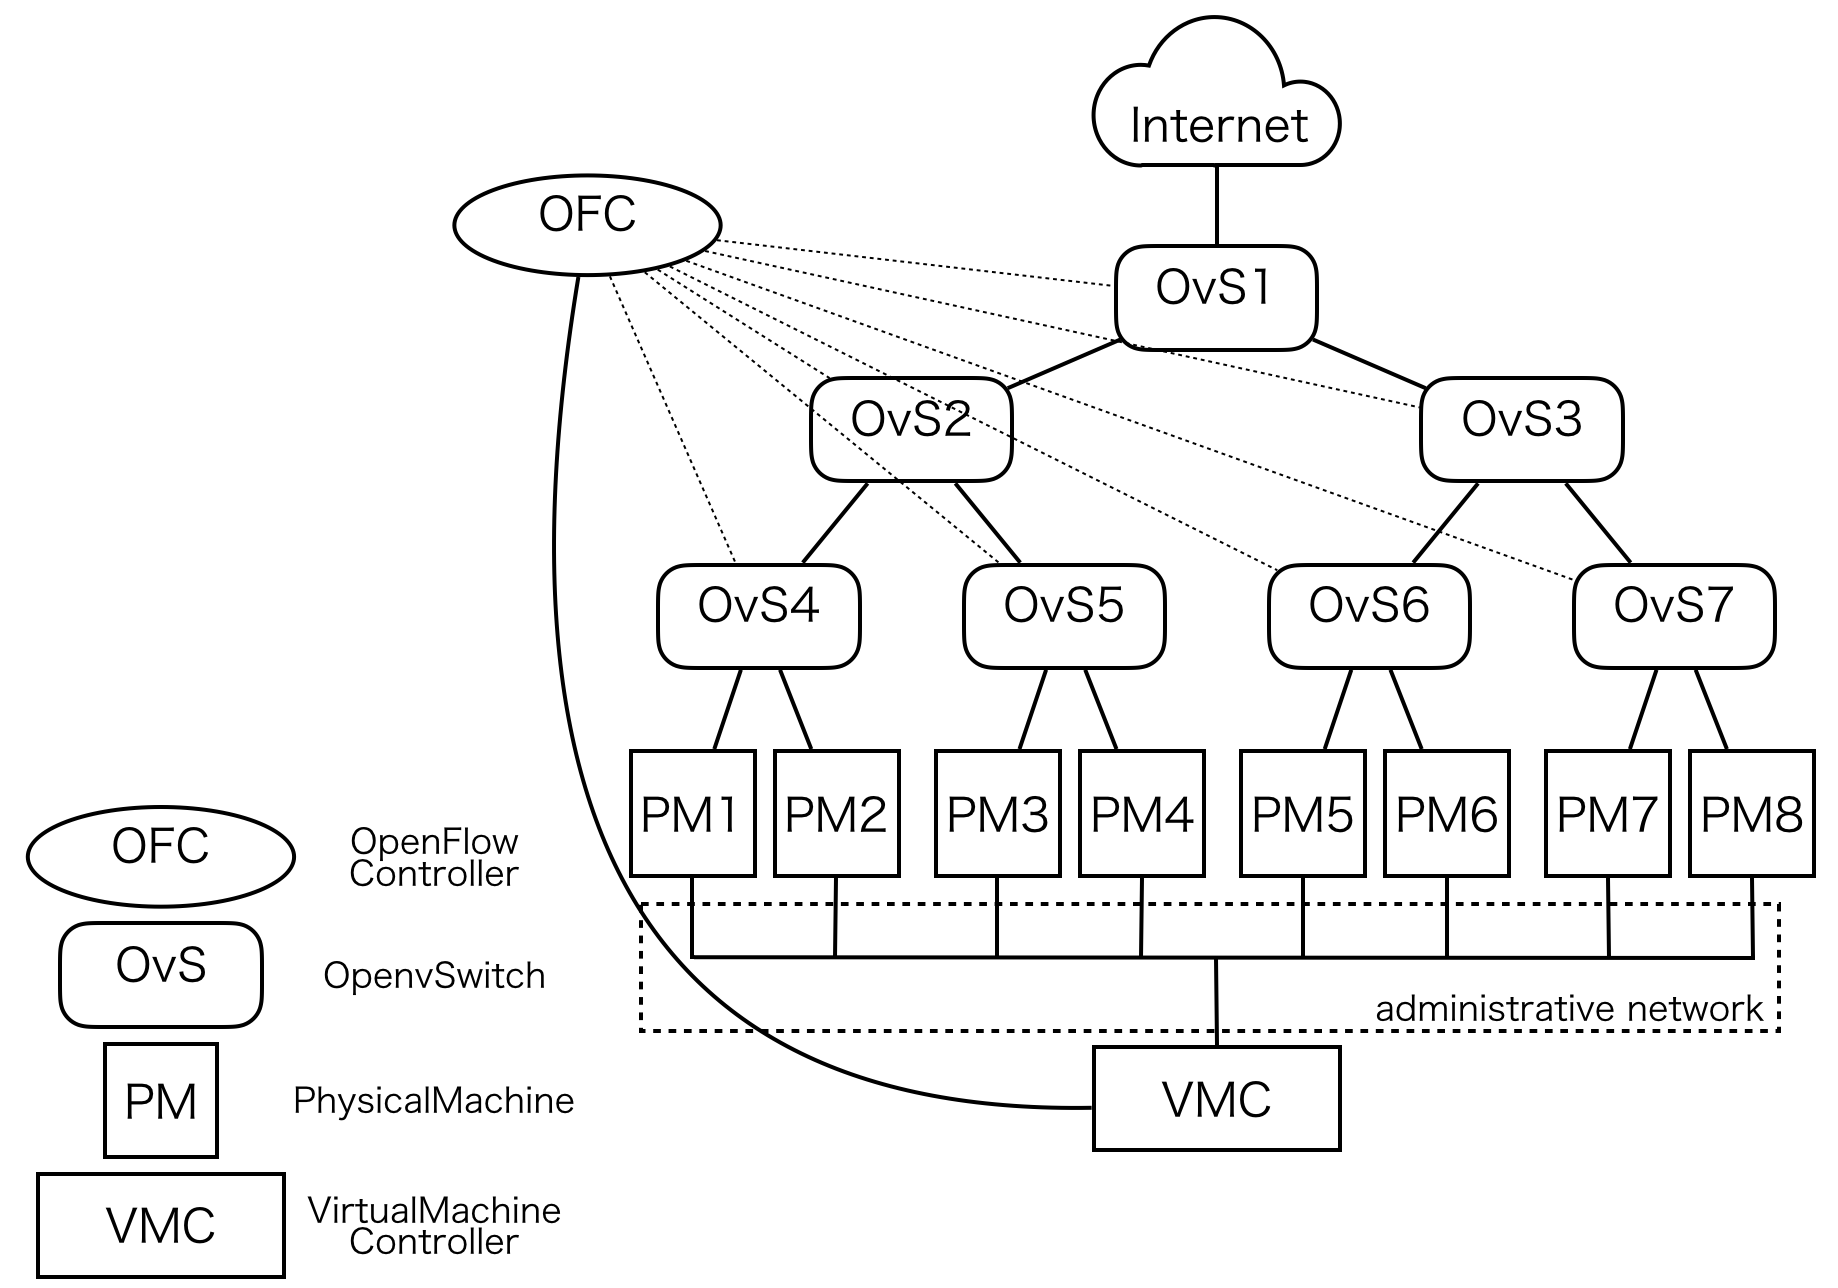
\includegraphics[width=8.5cm,bb=0 0 850 557]{fig/topology.png}
	\caption{テスト環境のアーキテクチャ}
	\label{fig:topology}
\end{figure}


\subsection{テスト環境のアーキテクチャ}\label{subsec:arch}
\ref{subsec:requirement}節で述べたように,多数の物理マシンや仮想マシンの
状態管理,および制御を個別に行うことは困難である.そこで,本研究では,
仮想マシンや仮想マシンを起動する物理マシンを一元管理する仮想マシンコン
トローラ(VMC)を実現する.また,KVMを用いた仮想マシンの移動にはNFSを利
用する必要があり,一般にNFSの利用はローカルネットワークであることが望
ましい.そこで本テスト環境では,図\ref{fig:topology}に示すように,ユー
ザがサービス利用のために利用するネットワークとは異なる管理ネットワーク
を設け,すべての物理マシンを管理ネットワークにも接続する.そして,この
管理ネットワークにVMCを接続することで,後述する負荷状況やIPアドレス,
およびルーティングの管理を容易にする.


\subsection{負荷状況の把握}
負荷状況の指標として,各物理マシンのCPU使用率とメモリ使用
率,各スイッチのトラフィック量を取得する.物理マシンのCPUおよびメモリ使用量は
物理マシンの/procディレクトリに格納されているファイルからリソース
使用量を計算するプログラムを実装し,一定間隔(デ
フォルトは10秒毎)で実行してその値をデータベースに格納する.
また,トラフィック量の取得には,各OvSが計測している統計情報を元に各OvS全体,ポート毎のトラフィック量をそれぞれ取得する.
そして,これらの情報をOpen Flow ControllerであるOFCに送信し,OFCのデータベースに格納する.
VMCはOFCのデータベースにアクセスを行うことで,トラフィック量を取得することができる.

%トラフィック量,特定の
%OvSのポートのトラフィック量,各物理マシンへのトラフィック量を取得し,
%OvSを制御するOpenFlowController(OFC)に転送する.しかし,OFCに統計情報
%を送り続けると,ネットワークに負荷がかかってしまうため,定期的に情報を
%取得し,転送を行う.

\subsection{IPアドレスとルーティング管理}
テスト環境では,使用中のIPアドレスをVMCで動作するデータベースで管理し,仮想マシンの
起動や複製,移動時に次の手順で決定し,実際に設定する.
まず,移動先物理マシンが所属するネットワークアドレスを調べ,使用中のIPアドレス一覧を
取得する.次に,ネットワークアドレス,ブロードキャストアドレス,使用中のIPアドレスを
除きランダムで決定しする.最後に,起動,複製,移動後の仮想マシンのifconfig,route
コマンドを使用してIPアドレスとデフォルトルートを設定する.

次に,異なるネットワークに仮想マシンの移動や複製を行う場合,OpenFlowを
利用し,経由するOvSの設定を変更することで,パケットの転送経路を変更す
る.具体的には,仮想マシンを移動する時,OFCはすべてのOvSのルーティング
情報を保持ししているため,移動前アドレスのルーティングテーブルが存在す
るOvSを探索し,パケットを転送するポートを変更すると同時にパケットの送
信先アドレスを変更する.そして,移動後の仮想マシンから戻るパケットに関
しては,送信元アドレスを移動前のアドレスに書き換えて送信する.また,仮
想マシンを複製する時には,移動と同様の処理を1/2の割合で実行すること
により,ラウンドロビンで負荷を分散する.

\begin{table}[tb]
	\centering
	\caption{APIで使用できる機能}
	\label{tab:api}
	{
		\small
		\begin{tabular}{|l|l|} \hline
		仮想マシンの起動 & http://IPaddress:8000/vmStart?id\\ \hline
		複製 & http://IPaddress:8000/clone?from?to\\ \hline
		移動 & http://IPaddress:8000/migrate?from?to\\ \hline
		リソースの取得 & http://IPaddress:8000/getResource?id\\ \hline
		\end{tabular}
	}
\end{table}
\subsection{複数マシンの管理}
\ref{subsec:arch}で述べた通り,VMCを使用することで,多数の物理マシンや仮想マシンの状態管理や制御を個別に行うことが可能になる.
本テスト環境の利用者は,VMCで立ち上げたWebサーバにアクセスするだけで,各物理マシンの操作が可能になる.
また,アルゴリズムのテストを行うために,表\ref{tab:api}に示す負荷状況の把握や仮想マシンの操作が行えるWebAPIを実装した.
仮想マシンの起動では,指定したidの物理マシンに仮想マシンを起動する.
仮想マシンの複製と移動では,fromに指定したidの仮想マシンをtoに指定したidの物理マシンに複製・移動を行う.
リソースの取得では,idに指定した物理マシン,仮想マシンのリソースをjson形式で取得する.
このWebAPIを使用することで,仮想マシンの起動,移動,複製と各物理マシンのリソースの取得を行うことが可能になる.

%3

%4
% \section{本研究について}

% 本研究では,主にマイグレーションやクローンなどの仮想化技術とユーザに意識させないネットワークの構築が必要となる.
% まずは仮想化技術について述べる.

% \subsection{仮想化技術について}

% \begin{table}[tb]
% 	\centering
% 	\caption{RaspberryPi2 ModelBの性能}
% 	\label{tab:rpi2}
% 	{
% 		\small
% 		\begin{tabular}{|c|c|} \hline
% 		CPU & ARM Cortex-A7 クアッドコア 900MHz\\ \hline
% 		メモリ & 1GB\\ \hline
% 		ネットワーク & 10/100Mbpsイーサネット\\ \hline
% 		電源 & 900mA(4.5~5.5W)\\ \hline
% 		\end{tabular}
% 	}
% \end{table}
% \begin{table}[tb]
% 	\centering
% 	\caption{APIで使用できる機能}
% 	\label{tab:api}
% 	{
% 		\small
% 		\begin{tabular}{|l|l|} \hline
% 		仮想マシンの起動 & http://IPaddress:8000/vmStart/id\\ \hline
% 		クローン & http://IPaddress:8000/clone/from\_id/to\_id\\ \hline
% 		マイグレーション & http://IPaddress:8000/migrate/from\_id/to\_id\\ \hline
% 		リソースの取得 & http://IPaddress:8000/getResource/id\\ \hline
% 		\end{tabular}
% 	}
% \end{table}
% \begin{figure}[tb]
% 	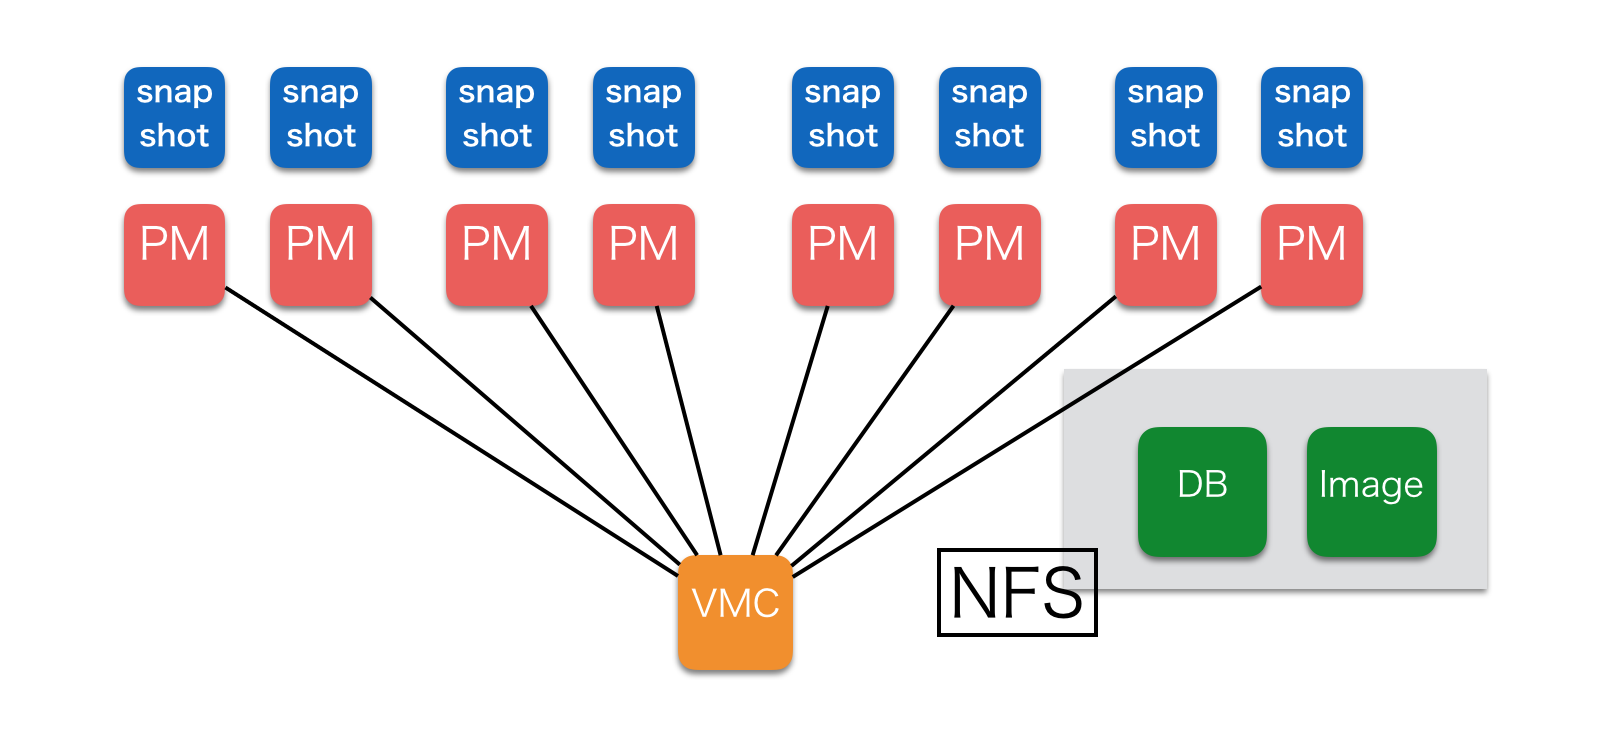
\includegraphics[width=8.5cm,bb=0 0 799 373]{fig/nfs.png}
% 	\caption{NFS}
% 	\label{fig:nfs}
% \end{figure}



% はじめに,今回使用するRaspberryPiの基本性能について説明する.
% 今回,RaspberryPiはRaspberryPi2 ModelBを使用する.
% RaspberryPiで使用するOSはRaspberryPi専用のLinux系OSであるRaspbianJessieLiteを使用する.
% RaspberryPi2 ModelBの性能は表\ref{tab:rpi2}の通りである.
% RaspbianJessieLiteでは,仮想化の機能が提供されていないので,仮想マシンの操作(e.g.起動,マイグレーション,クローン)を行うことができるvirtのようなソフトウェアを使用することができない.
% そのため,クローンやマイグレーションの操作をRaspbianJessieLiteで実行できる機能を提供する必要がある.
% アルゴリズムのテストを行うには,物理マシンや仮想マシンのリソースの取得,負荷分散のためのクローンやマイグレーションといった機能が必要である.
% しかし,仮想マシンの操作は非常に複雑である.
% 本環境では,仮想マシンを起動する物理マシンが多数存在する.
% それぞれの物理マシンのIPアドレスを記憶,またはモニターに繋げ,操作するのは非常に手間がかかってしまう.
% そこで,本研究では,仮想マシンの操作を統括的に行うことができる仮想マシンコントローラ(VMC)を実装した.
% 本テスト環境の利用者は,このVMCに接続するだけで,仮想マシンの操作が可能になる.
% 仮想マシンの操作を行うAPIとして,表\ref{tab:api}に示す機能を提供する.
% このAPIはRESTfulなAPIなので,どのプログラミング言語でも使用することが可能である.
% この機能を使用し,開発したアルゴリズムのプログラムを作成することで,アルゴリズムのテストを行うことを可能にする.
% 各物理マシンのリソースとして,CPU使用率とメモリ使用率を取得する.
% これらのリソースを各物理マシンで自動で定期的に取得を行い,データベースに格納する.
% また,全ての物理マシンとVMCをNFSを用いてデータベースを共有し,必要な時にVMCから情報を取得できるようにする.
% NFSを使用する理由は他にもある.
% 表\ref{tab:rpi2}に示すように,RaspberryPiのネットワーク転送速度は100Mbpsが限界である.
% したがって,数GBあるイメージファイルを転送すると,数十秒かかってしまい,さらにネットワークに負荷がかかってしまう.
% そこで,スナップショットを利用して,転送するイメージファイルの容量を削減する.
% スナップショットとは,あるイメージファイルの差分のみを保存する方法である.
% スナップショットを使用するには,元のイメージファイルと差分ファイル両方にアクセスできる必要がある.
% そこで,NFSを利用して,元のイメージファイルを全ての物理マシンと共有し,差分ファイルのみを転送することで,イメージファイルの転送を可能にする.
% 各物理マシンとVMCの関係は,図に表すと図\ref{fig:nfs}のようになる.

% \subsection{ネットワーク構築について}
% \begin{figure}[tb]
% 	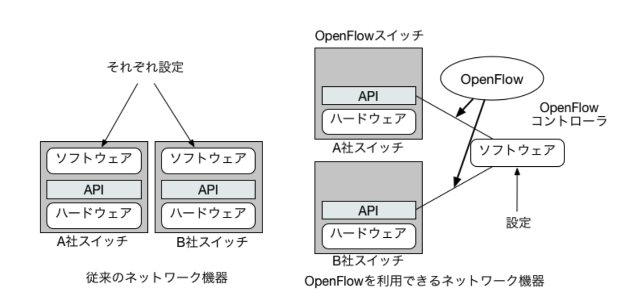
\includegraphics[width=8.5cm,bb=0 0 626 302]{fig/openflow.png}
% 	\caption{ネットワーク機器の違い}
% 	\label{fig:openflow}
% \end{figure}
% \begin{table}[tb]
% 	\centering
% 	\caption{アクション一覧}
% 	\label{tab:action}
% 	{
% 		\small
% 		\begin{tabular}{|c|l|} \hline
% 		アクション & 説明\\ \hline \hline
% 		Forward & パケットを指定のポートに転送する\\ \hline
% 		Drop & パケットを破棄する\\ \hline
% 		Field-Modify & パケットの指定したフィールドを書き換える\\ \hline
% 		Enqueue & パケットを指定したキューに格納する\\ \hline
% 		\end{tabular}
% 	}
% \end{table}
% \begin{figure}[tb]
% 	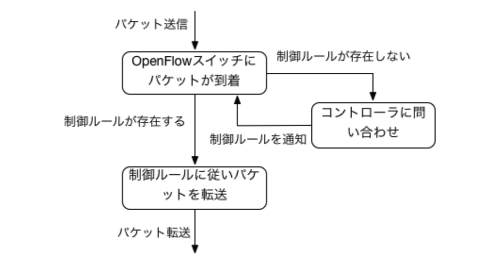
\includegraphics[width=8.5cm,bb=0 0 497 268]{fig/openflow_basic_action.png}
% 	\caption{OpenFlow基本動作}
% 	\label{fig:basic_action}
% \end{figure}

% RaspberryPiを用いてマルチテナント環境を実現するには,仮想マシンの生成や破棄,マイグレーションやクローンを行う時に発生するネットワーク構成の変更要求に柔軟に対応するネットワークの構築が必要となる.
% マルチテナントではSoftware Defined Network(SDN)\cite{sdn}の概念を用いて,ネットワークが構成されている.
% 本研究では,ネットワークの構築にOpenFlowを用いて実装を行なった.
% \subsubsection{OpenFlowとは}
% OpenFlow\cite{opf}はSDNを実現する有力なプロトコルと言われている.
% 図\ref{fig:openflow}に示すように,従来のネットワーク機器とOpenFlowに対応したネットワーク機器は仕組みが異なる.
% 従来のネットワーク機器はハードウェア制御のためのAPIが非公開であるが,OpenFlowはハードウェア制御のためのAPIが標準化されている.
% これにより,ハードウェアのAPIをユーザが自由に利用できるため,独自の機能の開発や実装を行うことが可能になる.
% また,従来のスイッチとは違い,ハードウェアとソフトウェアが分離可能なため,図\ref{fig:openflow}のように,複数のネットワーク機器を1つの外部のソフトウェアから制御することが可能になった.
% OpenFlowでは,OpenFlowに対応したスイッチをOpenFlowSwitch(OFS),OFSを制御するソフトウェアのことをOpenFlowController(OFC)と呼ぶ.

% OpenFlowでは,OFSでデータの転送のみを行い,OFCが経路制御を行う.
% OpenFlowは条件にマッチしたパケットに対し,表\ref{tab:action}に示すアクションを実行する.
% 条件とアクションの組み合わせをフローといい,それが格納されているものをフローテーブルと呼ぶ.

% 次に,OpenFlowの基本動作を図\ref{fig:basic_action}に示す.
% OFSにパケットが到達すると,OFSが保持するフローテーブルを確認し,そのフローテーブルに記述されている通りにパケットを転送する.
% フローテーブルにフローが記述されていれば,フローに従いパケットの転送を行うが,フローが記述されていない場合,OFCに制御ルールの問い合わせを行い,OFSがOFCから返ってきたフローをフローテーブルに追加する.
% 以上のようにOpenFlowが動作し,パケットの転送が行われる.

% \subsubsection{クローンの場合}
% クローンを行なった場合には,自動でスケールアウトを行うようにする.
% スケールアウトを実現するには,クローンされる仮想マシンとクローンにより生成された仮想マシンに対してネットワーク構成を変更し,OpenFlowスイッチをロードバランサとして機能させることで実現させる.
% 通常,ロードバランサはあらかじめロードバランスを行うことを想定し,ロードバランスする仮想マシンを用意し,ロードバランサを設置する.
% そのため,ロードバランスを行わない場合にも,仮想マシンを待機させておく必要が生じる.
% しかし,本研究ではロードバランスの要求が発生した時に,ロードバランサと仮想マシンの調達を行うことで,無駄なリソースの消費を無くす.

% クローンを行う場合は,次のように処理を行う.
% クローンが完了した通知をOFCが受け取った時,同時にクローン元の仮想マシン(VM1)とクローンよって生成された仮想マシン(VM2)のIPアドレスを受け取る.
% 次に接続している全てのOFSのフローテーブルを取得し,フローテーブルにVM2のIPアドレスに関するフローが存在するかどうかの判別を行う.
% VM1とVM2のIPアドレスの比較を行い,フローが存在した場合にはそのフローの優先度を下げ,特定のOVSにロードバランサの機能を付与する.
% ロードバランサの機能を付与した後は,VM1とVM2に送信元IPアドレスごとにパケットをラウンドロビンによって割り振る.
% VM2にパケットを転送する場合には,送信元を偽装し,VM1からのパケットであるかのように振る舞う.
% ロードバランスを行う前のセッションは,クローンによって情報が引き継がれるため保持されている.
% しかし,ロードバランス後のセッションは保障されない.
% そこで,接続元IPアドレスごとに転送先仮想マシンを割り当てることで,セッションの維持を行う.


% \subsubsection{マイグレーションの場合}
% マイグレーションでは物理マシンに存在する仮想マシンをIPアドレス,MACアドレス共にそのまま別の物理マシンへ移動するため,異なるネットワークに属する物理マシンへマイグレーションを行うことができない.
% そのため,マイグレーションは負荷が高い物理マシンの負荷を下げるために行われるが,ネットワーク内のすべての物理マシンの負荷が上がってしまった場合には,以上の理由により,マイグレーションを行うことができなくなってしまう.
% そこで,マイグレーションが行われた仮想マシンのIPアドレスをマイグレーション先の物理マシンと同じネットワークのIPアドレスに新たに割り当てる.
% 加えて,フローテーブルを書き換え,特定のIPアドレスのみを判別し,移動されたマシンにパケットを届けるという動作を行うことで,異なるネットワークにマイグレーションを行うことを可能にする.

% マイグレーションを行う場合は,次のように処理を行う.
% マイグレーションが完了した通知をOFCが受け取った時,同時に移動前と移動後の仮想マシンのIPアドレスを受け取る.
% OFSのフォローを取得し,フローテーブルに移動先IPアドレスに関するフローが存在するかの判別を行う.
% フローが存在した場合にはそのフローの優先度を下げ,存在しない場合にはフローの追加を記述する.
% 優先度を下げることで,マイグレーションされた仮想マシン宛への専用のフローを優先して選択することが可能になる.
% フローの追加には,アクションにIP/MACアドレスを書き換えることで偽装し,移動前の仮想マシンへの転送を移動後の仮想マシンへ転送する.

% \subsubsection{トラフィック量の取得}
% \begin{table}[tb]
% 	\centering
% 	\caption{統計情報\cite{openflow}}
% 	\label{tab:total_info}
% 	{
% 		\small
% 		\begin{tabular}{|l|c|} \hline
% 		カウンター & Bits\\ \hline \hline
% 		\multicolumn{2}{|c|}{フローテーブルごと}\\ \hline
% 		有効エントリー数 & 32\\
% 		パケットルックアップ数 & 64\\
% 		パケットマッチ数 & 64\\ \hline
% 		\multicolumn{2}{|c|}{フローごと}\\ \hline
% 		受信パケット数 & 64\\
% 		受信バイト数 & 64\\
% 		フローが作られてからの経過時間(s) & 32\\
% 		フローが作られてからの経過時間(ns) & 32\\ \hline
% 		\multicolumn{2}{|c|}{ポートごと}\\ \hline
% 		受信パケット数 & 64\\
% 		転送パケット数 & 64\\
% 		受信バイト数 & 64\\
% 		転送バイト数 & 64\\
% 		受信ドロップ数 & 64\\
% 		転送ドロップ数 & 64\\
% 		受信エラー数 & 64\\
% 		受信フレームアライメントエラー数 & 64\\
% 		受信オーバーランエラー数 & 64\\
% 		受信CRCエラー数 & 64\\
% 		コリジョン数 & 64\\ \hline
% 		\multicolumn{2}{|c|}{キューごと}\\ \hline
% 		転送パケット数 & 64\\
% 		転送バイト数 & 64\\
% 		転送オーバーランエラー数 & 64\\ \hline
% 		\end{tabular}
% 	}
% \end{table}
% マイグレーションやスケールアウトする時の指標としてトラフィック量を利用するため,OpenFlowに格納されている情報を取得する.
% フローの構成要素の一つに,統計情報というものがある.
% 統計情報はOpenFlowスイッチに備えられているカウンターであり,表\ref{tab:total_info}に示す情報を利用することができる.
% 本研究では各OFSのトラフィック量,特定のOFSのポートのトラフィック量,各物理マシンへのトラフィック量を取得可能にする.
% トラフィック量を取得する時にはOFCに統計情報を送り続けることになるので,転送速度が低下してしまう.
% したがって,トラフィック量を10秒ごとに取得し,要求を受け取った時に出力を行うようにすることで,転送速度の低下を防ぐ.

%5
\section{評価}

本節では,本テスト環境の妥当性についての評価を行う.
今回,実験は図\ref{fig:topology}のような環境で行う.
\begin{table}[tb]
	\centering
	\caption{サーバを通信する時の経由するOvSの数}
	\label{tab:route}
	\vspace{4mm}
	{
		\begin{tabular}{ c c c } \hline
      route & 通信間 & 経由するOvS数 \\ \hline \hline
      1 & Server1 $\longleftrightarrow$	Server2 & 1 \\ \hline
      2 & Internet $\longleftrightarrow$ Server1 & 3 \\ \hline
      3 & Server1 $\longleftrightarrow$	Server3 & 3 \\ \hline
      4 & Server1 $\longleftrightarrow$	Server8 & 5 \\ \hline
		\end{tabular}
	}
\end{table}

仮想マシンの複製や移動が発生した場合のルーティングが行われるまでの転送時間をiperf\cite{iperf}を用いて計測した.
最大TCPセグメントサイズを128Byte/256Byte/512Byte/1024Byte/1400Byteの5段階に設定し,表\ref{tab:route}に示す状況においてそれぞれ計測した.
仮想マシンの移動を実際に行うと,仮想マシンの移動の発生から完了,その後にネットワーク構成変更まで平均して合計約38秒かかった.
仮想マシンの移動の実験には,図\ref{fig:topology}の環境で1つのスイッチを経由するルートで行なった.
作成したAPIを用いて仮想マシンの移動を行うと,表\ref{tab:times}のような結果になった.
\begin{table}[tb]
	\centering
	\caption{仮想マシンの移動の合計時間内訳}
	\label{tab:times}
	\vspace{4mm}
	{
		\begin{tabular}{ c c } \hline
      内訳 & 時間 \\ \hline \hline
      仮想マシンの移動の開始から完了 & 約33秒 \\
			ネットワーク構成変更 & 約3秒 \\
			遅延時間 & 約2秒 \\ \hline
		\end{tabular}
	}
\end{table}
仮想マシンの移動の実行は単体テストの際に約33秒かかる事が判明している.
仮想マシンの移動の開始から完了するまでは,移動元の仮想マシンが動作中であるため,ネットワークが切れることはなく,
仮想マシンの移動の完了後,移動元の仮想マシンが停止し,ネットワークの構成変更時に初めてネットワークが遮断される.
実験の結果,ネットワークの構成変更には約3秒かかる事が結果として得られている.
その他にかかる約2秒はVMCからOFCへ,移動が発生したと通知する時にかかる通信による遅延時間だと考えられる.
結果,仮想マシンの移動の発生からネットワークの構成変更までに合計約38秒の時間がかかるが,pingが通じなくなり,ネットワークが遮断される時間は約4秒であった.
仮想マシンの複製実行時には,複製が実行されてから,VM1へIPアドレスを変化しながらアクセスを繰り返し,VM2へ初めてリクエストが送信されるまでには約47秒の時間がかかった.
仮想マシンの複製の実験においても,図\ref{fig:topology}の環境で1つのスイッチを経由するルートで行なった.
作成したAPIを用いて仮想マシンの複製を行うと,表\ref{tab:ctimes}のような結果になった.
仮想マシンの複製においても,複製に約41秒ほど,ネットワークの構成の変更に約4秒,仮想マシンの移動の場合と同原因と思われる遅延時間が約2秒発生した.
仮想マシンの移動の場合とは異なり,仮想マシンの複製では複製後も,複製元仮想マシンが動作しているため,ネットワークが遮断されることがなかった.

\begin{table}[tb]
	\centering
	\caption{仮想マシンの複製の合計時間内訳}
	\label{tab:ctimes}
	\vspace{4mm}
	{
		\begin{tabular}{ c c } \hline
      内訳 & 時間 \\ \hline \hline
      仮想マシンの移動の開始から完了 & 約41秒 \\
			ネットワーク構成変更 & 約4秒 \\
			遅延時間 & 約2秒 \\ \hline
		\end{tabular}
	}
\end{table}


ネットワークの速度は図\ref{fig:graph}の示す結果となった.
\begin{figure}[tb]
	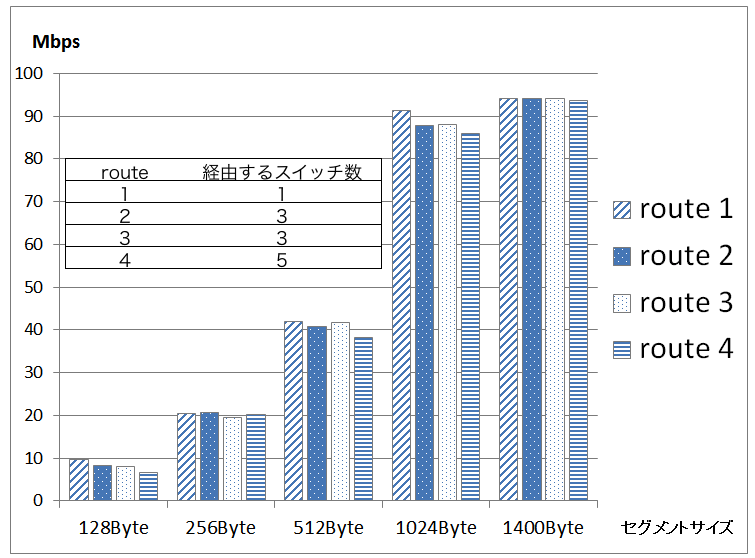
\includegraphics[width=8.5cm,bb=0 0 755 558]{fig/graph.png}
	\caption{ネットワーク速度}
	\label{fig:graph}
\end{figure}

route1とroute4を比較すると分かるように,経由するOvSの数によって僅かに転送速度が低下する.
また,図\ref{fig:graph}で示す,セグメントサイズが1024Byteと1400Byteにした際のトラフィック速度に大きな変化は見られなかった.

トラフィック量の取得についてもiperfを用いて検証を行い,iperfでネットワークに負荷を加え,本研究で実装したトラフィック量取得の機能を用いて
接続されるOvS全てのトラフィック量を取得し,続いて,ネットワーク全体のトラフィック量を取得を行った.
これら値は,

OvS1+OvS2+OvS3+...+OvSx = ネットワーク全体のトラフィック量 = iperfで転送したトラフィック量

となる事が明白であり,本環境において,上記した式の結果を得ることができたため,正確な値であると言える.

セグメントサイズが1024Byteと1400Byteにした際のトラフィック速度に大きな変化は見られなかったが,RasPIのイーサネットは10/100Mbps
ポートであるため100Mbps以上の転送速度を得ることはできない.したがって正確な値であると測定でき,仮に1Gbpsの転送速度性能を持つスイッチであれば
10倍の転送速度を期待でき,仮想マシンの移動や複製にかかる時間も低下する.
仮想マシンの移動や複製におけるネットワークの構成変更にかかる処理時間は,RasPIより高性能な物理マシンでは高速になる.
実際に1Gbpsポート,Intel Core 2 DuoであるCPUを搭載した高性能物理マシンにおいて,仮想マシンの移動と複製を行うと表\ref{tab:c2d}の結果となった.
\begin{table}[tb]
	\centering
	\caption{高性能物理マシンでの実行時間}
	\label{tab:c2d}
	\vspace{4mm}
	{
		\begin{tabular}{ c|c c } \hline
      & 移動 & 複製  \\ \hline \hline
      実行時間 & 2.23秒 & 6.01秒\\ \hline
		\end{tabular}
	}
\end{table}
表\ref{tab:c2d}に示すように,仮想マシンの移動では本環境のおよそ15分の1の転送速度,複製ではおよそ12分の1の転送速度であった.
この差はネットワーク速度,また処理性能の差により発生するものであり,本環境を高性能物理マシンで実行すると同等の実行時間を得ることができる.

また,route1とroute4のように経由するOvSの数によって転送速度が低下する問題についても本環境に限らず生じる現象であり,
本研究において実装したOFCによって発生する低下は非常に少ないと考えられ,ボトルネックになることは無いと言える.

% <時間経過のCPU使用率とメモリ使用率の推移>

% <機能の所要時間>

% <環境の差でどのような影響が出るか>

%6
\section{関連研究}
% 関連研究:AWSとOpenStackについて
本研究の関連研究として,AWSやOpenStackなどのクラウド環境を構築できるIaaSが挙げられる.
しかし,これらのサービスでは,本研究の目的であるインフラ提供者とサービス提供者の要求を満たすことができない.

\begin{figure}[tb]
	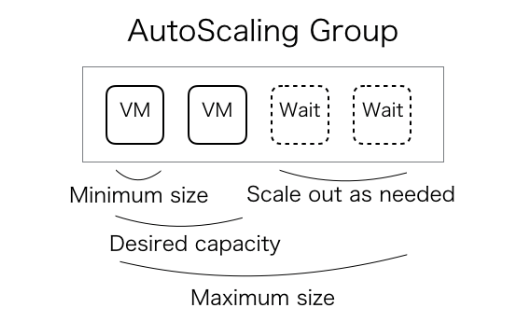
\includegraphics[width=8.5cm,bb=0 0 513 320]{fig/autoscaling.png}
	\caption{AutoScaling}
	\label{fig:autoscaling}
\end{figure}
\subsection{AWS\cite{aws}}
IaaSのクラウドコンピューティングサービスであるAWSでは,仮想マシンと同様のインスタンスをサービス提供者にリソースとして提供している.
AWSには様々なサービスが提供されており,Amazon Elastic Compute Cloud(Amazon EC2)というインスタンスを提供するサービスや,Amazon Simple Storage Service(Amazon S3)というクラウドストレージを提供するサービスが存在する.
サービスの中には,AutoScalingという負荷がかかった場合にEC2インスタンスを自動で増減させ,スケールアウト/スケールインを行う機能や,Elastic Load Balancingというロードバランスを行う機能が提供されている.
AutoScalingは,図\ref{fig:autoscaling}に示すように,AutoScaling Groupを作成し,EC2インスタンスの最小数と最大数を設定し,処理負荷がかかった場合に,待機状態のEC2インスタンスを立ち上げ,ロードバランスを行い,負荷分散を行なっている.
また,処理負荷が少なくなった場合には,EC2インスタンスを待機状態にし,リソースを有効活用できるようにしている.
しかし,このAutoScaling Groupは異なるネットワークを跨いで作成することはできない.
したがって,ロードバランスを行う仮想マシンのネットワークは同一である必要があり,ネットワーク内のすべてのEC2インスタンスが過負荷状態になってしまった場合には対応できない.
また,事前に設定したEC2インスタンスの最大数を超える処理負荷がかかってしまった場合,全てのEC2インスタンスが正常に起動しなくなってしまうことがある.

加えて,AWSはEC2インスタンスを起動している物理マシンのリソース情報はブラックボックスになっており,実際に計測することができない.
また,物理マシン上でどのようにEC2インスタンスが動作しているか,トラフィック量の取得が不可能など,テスト環境としては不明瞭な点が多い.
したがって,AWSでテストを行うと,実際の環境で動作した時の予測をすることができないといった問題点が存在する.

% \begin{figure}[tb]
% 	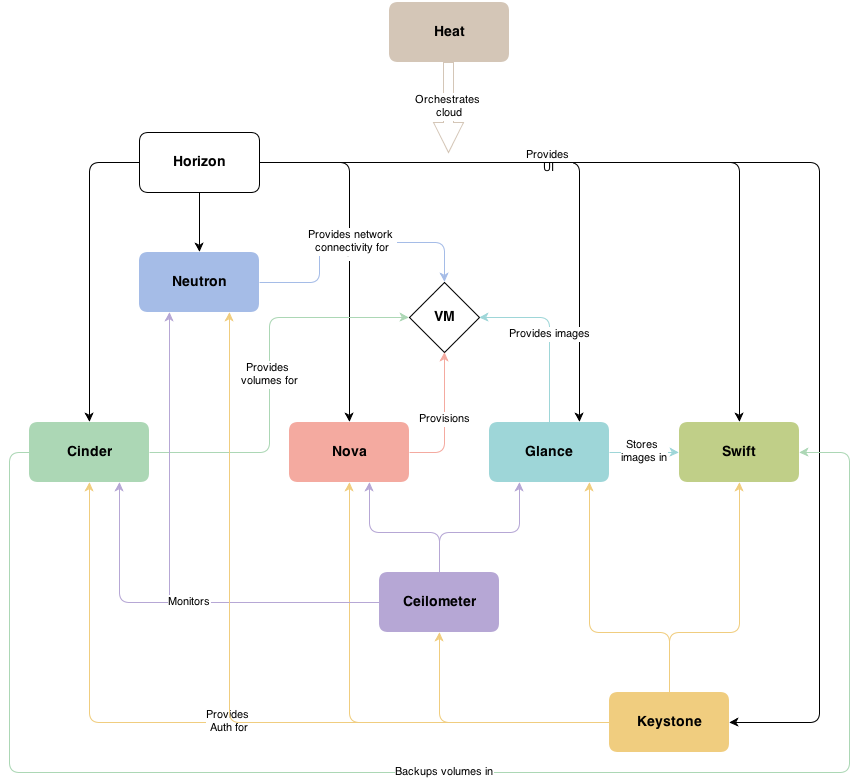
\includegraphics[width=8.5cm,bb=0 0 859 782]{fig/openstack.png}
% 	\caption{OpenStackのアーキテクチャ}
% 	\label{fig:openstack}
% \end{figure}
\subsection{OpenStack\cite{openstack}}
OpenStackはオープンソースで開発されているクラウド環境構築用のソフトウェア群である.
OpenStackでは,仮想マシンとストレージ,ネットワークといったリソースを提供するクラウド環境を構築することが可能である.
OpenStackは様々なコンポーネントの組み合わせで成り立っている.
中でも,仮想マシンを管理するNovaや仮想ネットワークを提供するNeutronが本研究と関連している.
OpenStackでは仮想マシンを起動,停止や移動を行うことができるが,仮想マシンの複製はリンククローンしか使えず,ネットワークと同期して仮想マシンの複製を行うことはできない.
また,性能を上げる方法として,物理マシンの性能を上げるスケールアップは行うことができるか,スケールアウトは行うことができない.
したがって,サービス提供者の自身のサービスの最大負荷見積もりという要求を満たすことができない.
また,特定の物理マシンのリソースの取得や特定のスイッチのトラフィック量を取得することができないといった問題があるため,アルゴリズムのテストを行うには不十分であると言える.

% 本研究と同じように,RaspberryPiを用いたデータセンタ環境の構築を行う論文は多数存在していたが,インフラ提供者,サービス提供者向けの論文は存在していない.
% 具体的にはリソースの取得や,スケールアウト,仮想マシンに同期して変更を行うネットワークの構築をRaspberryPi上で行なっている研究である.
% したがって,関連研究から本研究の有用性について述べることとする.

% \subsection{高速マイグレーションを利用した仮想マシン配置最適化システムの検討\cite{thesis1}}
% \begin{figure}[tb]
% 	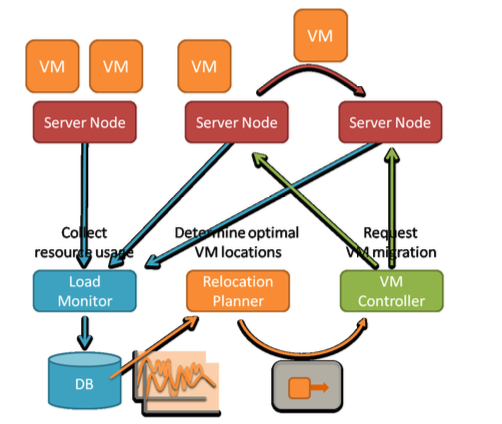
\includegraphics[width=8.5cm,bb=0 0 502 424]{fig/thesis1.png}
% 	\caption{仮想マシン集約システムの概要}
% 	\label{fig:thesis1}
% \end{figure}
% \begin{figure}[tb]
% 	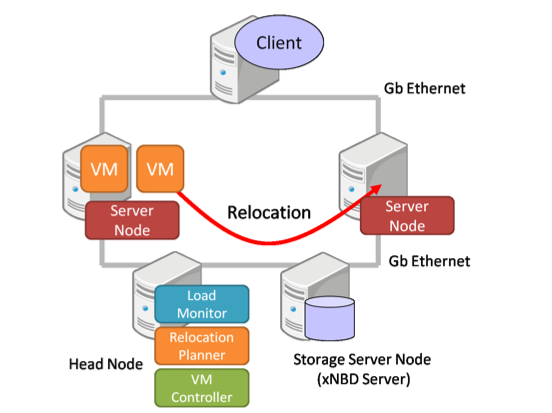
\includegraphics[width=8.5cm,bb=0 0 552 413]{fig/thesis2.png}
% 	\caption{実験環境}
% 	\label{fig:thesis1}
% \end{figure}
% \begin{figure}[tb]
% 	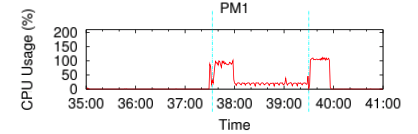
\includegraphics[width=8.5cm,bb=0 0 418 134]{fig/thesis3.png}
% 	\caption{物理マシンのCPU使用率}
% 	\label{fig:thesis3}
% \end{figure}
% \begin{figure}[tb]
% 	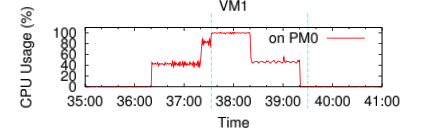
\includegraphics[width=8.5cm,bb=0 0 428 134]{fig/thesis4.png}
% 	\caption{仮想マシンのCPU使用率}
% 	\label{fig:thesis4}
% \end{figure}
% % アルゴリズム開発の例としてこのような研究が存在する.
% この研究では,データセンタの利用効率を高めるため,マイグレーションを利用した資源利用向上のための仮想マシンの再配置を行なっている.
% 仮想マシンの動的再配置機構に対し,ポストコピー型マイグレーションを適用することで,短時間で仮想マシンの再配置を可能にする.
% 図\ref{fig:thesis1}のように仮想マシン集約システムを構築することで,1秒程度で実行ホストの切り替えを可能にし,急激な負荷上昇に対応できる.
% 仮想マシン集約システムは資源消費量モニタ,再配置計画エンジン,VMコントローラから成っている.
% 監視対象の資源消費量として,物理マシンと仮想マシンのCPU消費量を取得している.
% 一定時間以上,物理マシンのCPU使用率が閾値を上回ると分散配置を,下回ると集約配置を行う.
% この研究の実験では,2台の仮想マシンを用い,以下のようなアルゴリズムを用いて再配置を実行している.
% \begin{itemize}
% \item ある物理マシンのCPU使用率が90\%であり,なおかつその物理マシン上にactiveな仮想マシン(CPU使用率が5\%以上の仮想マシン)が複数台存在する状態になると,その物理マシンは過負荷状態になったと定義する.
% \item また,物理マシンのCPU使用率が30\%未満の状態を,その物理マシンはidle状態であると定義する.
% \end{itemize}
% 再配置は以下のような条件で判断を行う.
% \begin{itemize}
% \item 物理マシンの過負荷状態を検知すると,その物理マシン上のactiveな仮想マシンに対して,1台をその物理マシンに残し,残りをidle状態の物理マシンに移動することを決定する.
% このときCPU使用率が最も高い仮想マシンをその物理マシンに残す.
% \item idle状態かつ仮想マシンをホストしている物理マシンが複数存在することを検知すると,それらidle物理マシン上の仮想マシンを1台のidle物理マシン上に集約することを決定する.
% このときCPU使用率が最も高いidle物理マシンを集約先とする.
% \end{itemize}
% 評価には以上の条件で仮想マシンの再配置を行い,仮想マシンのCPU使用率を操作し,検証を行った.
% その結果,物理マシンでは図\ref{fig:thesis3},仮想マシンでは図\ref{fig:thesis4}のようになった.
% したがって,このアルゴリズムでは仮想マシン集約システムが仮想マシンの負荷変動に追随して動的に配置を最適化できた.
% このような研究があり,以上のようなアルゴリズムであれば,本研究を用いて実験,評価が行うことができる.

% \subsection{The Glasgow Raspberry Pi Cloud:A Scale Model for Cloud Computing Infrastructures\cite{cloud2}}
% \begin{figure}[tb]
% 	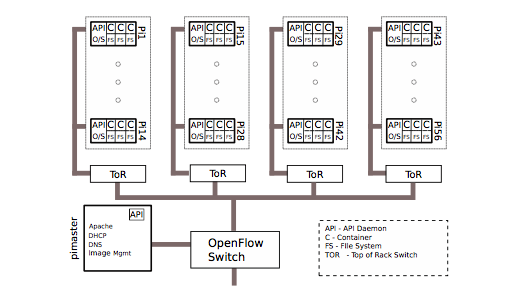
\includegraphics[width=8.5cm,bb=0 0 519 304]{fig/thesis5.png}
% 	\caption{システムアーキテクチャ}
% 	\label{fig:thesis5}
% \end{figure}
% % RaspberryPiでデータセンタ環境を模擬して,教育を目的としている.
% % このことからRaspberryPiでデータセンタ環境を模擬することは可能である.
% 一般的なクラウドデータセンタには,数万台のサーバを用いているため,教育機関や研究機関がそのサーバを構築することはコストの面で非常に難しい.
% そこで,この研究ではRaspberryPiを用いてクラウドテストベッドを構築し,費用の削減を行なっている.
% この研究では図\ref{fig:thesis5}のようなシステムアーキテクチャで構築されている.
% 結果から,クラウドテストベッドとして十分であるが,クローンやマイグレーション,スケールアウトやリソースの管理などの機能は明示されていない.
% しかし,この研究より,RaspberryPiでクラウドテストベッドを構築することは有用性あると言える.

%7
\section{まとめ}

クラウド環境で利用される仮想マシン再配置に関するアルゴリズムの開発は,データセンタなどを保持しない組織や個人では非常に困難であり,アルゴリズムを開発しても,実験や検証が困難な状況であった.
そこで,本研究では安価で小型なRasPIを用いることで,省スペースで低コストなデータセンタの構成を提案,構築した.
本環境では仮想マシンの移動や複製の仮想化技術を容易に利用可能な環境の構築を行なった.
結果,低コストでデータセンタの構成を実現した.

\subsection{今後の課題}
今後の課題を以下にまとめる.
本環境は全てCUIで動作するため,一目して,本環境の挙動が理解しにくい.
そこで,物理マシン,物理マシンで動作する仮想マシンを含めたネットワークのトポロジをグラフィカルに表示し,
ネットワークのトラフィック量もグラフを用いて表示可能なGUIの作成.
また本環境ではDHCPは実装しておらず,RasPIのIPアドレスはユーザが指定する必要があるため,DHCP機能の追加.
以上の機能の拡張が考えられる.
また,現在はVMC,OFC間の通信は現在sshを用いて行っており,コントローラ間の通信が全体の実行速度低下の原因となる.
そのため,コントローラ間の通信を行う独自のプロトコルの作成も今後の課題として挙げられる.

% % 謝辞
% \begin{acknowledgment}
% 研究への有益な示唆をいただいた,福田浩章先生に謝意を表する.
% \end{acknowledgment}

\begin{thebibliography}{10}


\bibitem{cloud1}
  Takahiro Hirofuchi, Hidemoto Nakada, Satoshi Itoh, Satoshi Sekiguchi, "Reactive Cloud: Consolidating Virtual Machines with Postcopy Live Migration", IPSJ Transactions on Advanced Computing Systems, Vol.5 No.2 86–98 ,2012

\bibitem{cloud2}
  広渕崇宏, 中田秀基, 伊藤智, 関口智嗣, "高速マイグレーションを利用した仮想マシン配置最適化システムの検討", 情報処理学会研究報告 IPSJ SIG Technical Report, Vol.2010-OS-115 No.14, 2010/8/4

\bibitem{testbed}
  H. Kim, J. Kim and Y. B. Ko, "Developing a cost-effective OpenFlow testbed for small-scale Software Defined Networking," 16th International Conference on Advanced Communication Technology, Pyeongchang, 2014, pp. 758-761.
  doi: 10.1109/ICACT.2014.6779064

\bibitem{virt}
  virt-manager website. https://virt-manager.org/ 2017/04/19

\bibitem{sdn}
  Open Netrowking Foundation website. https://www.opennetworking.org/ 2017/01/11

\bibitem{opf}
  Open Netrowking Foundation OpenFlow website. https://www.opennetworking.org/sdn-resources/openflow 2017-01-11

% \bibitem{openflow}
%   OpenFlow Switch Specification Version 1.0.0 (Wire Protocol 0x01) December 31, 2009. http://www.openflow.org/documents/openflow-spec-v1.0.0.pdf

% \bibitem{thesis1}
%   Fung Po Tso, David R. White, Simon Jouet, Jeremy Singer, Dimitrios P. Pezaros School of Computing Science, University of Glasgow, G12 8QQ UK, "The Glasgow Raspberry Pi Cloud: A Scale Model for Cloud Computing Infrastructures", 2013 IEEE 33rd International Conference on Distributed Computing Systems Workshops

\bibitem{iperf}
  iperf website.  https://iperf.fr/

\bibitem{aws}
  Amazon Web Services website. https://aws.amazon.com/jp/ 2017/04/19

\bibitem{openstack}
  OpenStack Documentation. https://docs.openstack.org/ 2017/04/19

%\bibitem{latex}
%Lamport, L.: {\em A Document Preparation System \LaTeX User's Guide \&
%  Reference Manual}, Addison Wesley, Reading, Massachusetts (1986).
% (Cooke, E., et al.訳:文書処理システム \LaTeX,アスキー出版局
%  (1990)).

%\bibitem{total}
%伊藤和人: \LaTeX トータルガイド,秀和システムトレーディング (1991).
%\bibitem{nodera}
%野寺隆志:楽々 \LaTeX,共立出版 (1990).

% \bibitem{okumura}
% 奥村晴彦:改訂第5版 \LaTeXe 美文書作成入門,
% 技術評論社(2010).

% \bibitem{companion}
% Goossens, M., Mittelbach, F. and Samarin, A.:
% {\it The LaTeX Companion},
% Addison Wesley, Reading, Massachusetts (1993).

% \bibitem{book1}
% 木下是雄:
% 理科系の作文技術,
% 中公新書(1981).

% \bibitem{book2}
% Strunk W. J. and White E.B.:
% {\it The Elements of Style, Forth Edition},
% Longman (2000).

% \bibitem{book3}
% Blake G. and Bly R.W.:
% {\it The Elements of Technical Writing},
% Longman (1993).

% \bibitem{book4}
% Higham N.J.:
% {\it Handbook of Writing for the Mathematical Sciences},
% SIAM (1998).

% \bibitem{webpage1}
% 情報処理学会論文誌ジャーナル編集委員会:
% 投稿者マニュアル(online),
% \urlj{http://www.ipsj.or.jp/journal /submit/manual/j\_manual.html}
% (2007.04.05).

% \bibitem{webpage2}
% 情報処理学会論文誌ジャーナル編集委員会:
% べからず集(online),
% \urlj{http://www.ipsj.or.jp/journal/manual /bekarazu.html}
% (2011.09.15).

\end{thebibliography}


%% 以下は無視されます

% \begin{biography}
% \profile{m}{情報 太郎}{1970年生.1992年情報処理大学理学部情報科学科卒.
% 1994年同大大学院修士課程了.同年情報処理学会入社.オンライン出版の研究
% に従事.電子情報通信学会,IEEE,ACM 各会員}
% %
% \profile{n}{処理 花子}{1960年生.1982年情報処理大学理学部情報科学科卒.
% 1984年同大大学院修士課程了.1987年同博士課程了.理学博士.1987年情報処
% 理大学助手.1992年架空大学助教授.1997年同大教授.オンライン出版の研究
% に従事.2010年情報処理記念賞受賞.電子情報通信学会,IEEE,IEEE-CS,ACM
% 各会員}
% %
% \profile{s}{学会 次郎}{1950年生.1974年架空大学大学院修士課程了.
% 1987年同博士課程了.工学博士.1977年架空大学助手.1992年情報処理大学助
% 教授.1987年同大教授.2000年から情報処理学会顧問.オンライン出版の研究
% に従事.2010年情報処理記念賞受賞.情報処理学会理事.電子情報通信学会,
% IEEE,IEEE-CS,ACM 各会員}
% %
% \end{biography}



\end{document}
